\documentclass{article}

\usepackage[english]{babel}
\usepackage[a4paper,top=2cm,bottom=2cm,left=3cm,right=3cm,marginparwidth=1.75cm]{geometry}

\usepackage{amsmath}
\usepackage{xcolor,graphicx}
\usepackage{hyperref}
\hypersetup{%
  colorlinks=true,
  breaklinks=true,
  linkcolor=blue,
  anchorcolor=black,
  citecolor=brown,
  filecolor=blue,
  menucolor=red,
  urlcolor=blue,
}
\usepackage[authoryear]{natbib}

% -------------
% Some commands
% -------------
\providecommand{\keywords}[1]{\textbf{\textit{Keywords---}} #1}

% -------------

\title{Is Stephen Curry really a guard? New perspective on players typology using functional data analysis}
\author{%
Steven Golovkine\thanks{MACSI, Department of Mathematics and Statistics, University of Limerick, Ireland \href{mailto:steven.golovkine@ul.ie}{steven.golovkine@ul.ie}}
\and
Edward Gunning\thanks{Department of Biostatistics and Epidemiology, University of Pennsylvania, USA \href{mailto:edward.gunning@pennmedicine.upenn.edu}{edward.gunning@pennmedicine.upenn.edu}}
}
\date{\today}

\begin{document}
\maketitle

\begin{abstract}
Your abstract.
\end{abstract}

\keywords{Basketball, Clustering, Functional Data Analysis, Sport Analytics}

% MAIN --------
%!TEX root=../main.tex
\section{Introduction} % (fold)
\label{sec:introduction}


Due to the increasing availability of detailed performance data, sport analytics is a growing field in recent times and receives a large interest in the statistics community. Concerning team sports, traditional approaches concern the prediction of game results based on team characteristics \citep{dixonModellingAssociationFootball1997,babootaPredictiveAnalysisModelling2019}. See \cite{horvatUseMachineLearning2020,bunkerApplicationMachineLearning2022} for recent reviews. Recently, the availability of tracking data allowed researchers to focus on more specific aspects of different sports, such as evaluating individual player performance in soccer \citep{pappalardoPlayeRankDatadrivenPerformance2019,decroosActionsSpeakLouder2019} or defensive performance on passing plays in American football \citep{schmidSimulatingDefensiveTrajectories2021}. Because of the data provided by the National Basket Association (NBA), basketball is an interesting sport to analyse from this perspective.

Basketball is a sport where two teams, consising of five players, compete each others. The objective of the game is to shoot a ball through the opponent's hoop while preventing the ball to go through your own hoop. Basketball has been widely studied from different perspective. Shooting movements have been analyzed in \cite{millerRelationshipBasketballShooting1996,liuChangesBasketballShooting1999,okazakiReviewBasketballJump2015}. Estimating game win probability, in-game win probability \citep{maddoxBayesianEstimationIngame2022} or possession outcomes \citep{cervoneMultiresolutionStochasticProcess2016}. Defense analysis \citep{csataljayEffectsDefensivePressure2013}. Spatial performance \citep{zuccolottoSpatialPerformanceAnalysis2023}. See \cite{ternerModelingPlayerTeam2021} for a review on performance analysis in basketball.

In basketball, the outcome of the game is greatly determined by the shooting accuracy. An important factor of a player's effectiveness is its ability to consistently make successful shots from various locations on the court. The analysis of shooting patterns can thus evaluate individual player performance but also help to develop team strategies. An important tool to analyse shooting patterns is shooting charts. Shooting charts are graphic representations of all the shots a player has taken and made across a season or a game. Shooting charts have been widely analysed in the basketball litterature. Most of the work in this area concern the modelling of the shooting charts as point process. To do so, the idea is to construct a count matrix of the number of shots by player on a discretized court, fit an intensity surface for each each player over the discretized court using a log-Gaussian Cox process and find a low-rank approximation of all players' intensity surface using non-negative matrix factorization \citep{millerFactorizedPointProcess2014,franksCharacterizingSpatialStructure2015}. Non-parametric estimation of the intensity surface is also considered in \cite{yinBayesianNonparametricLearning2022}. The low-rank approximation of the intensity surfaces is then used to summarize the shooting habits of NBA players as well as characterizing their efficiency. Some authors developed models that are not based on fitting an intensity surface for each player. For examples, \cite{reichSpatialAnalysisBasketball2006} proposed conditionally autoregressive models to consider spatial correlation and \cite{huZeroinflatedPoissonModel2023} fit a Bayesian zero-inflated Poisson model to model shoot attempts of players with different shooting preference. These methods allow us to summarize information about players but not compare different players. 

To compare players regarding their shooting behavior, specific methods have been developed. \cite{fuHoopInSightAnalyzingComparing2024} use (interactive) data visualization to analyze and compare basketball shooting performance.  \cite{huBayesianGroupLearning2021} use a log-Gaussian Cox process and define a similarity measure to compare the players. \cite{jiaoBayesianMarkedSpatial2021} proposes a Bayesian marked spatial point processes model to model the shots intensity. They study if the sucess rate of shot is higher at locations where players makes more shots and provide a clustering of players. \cite{wong-toiJointAnalysisField2022} analyzes shooting patterns among different players. They quantify the shooting patterns using a discretisation of the field by performing a Bayesian nonparametric mixture model to find latent clusters of players. \cite{yinAnalysisProfessionalBasketball2023} proposes a Bayesian nonparametric matrix clustering approach on estimated intensity maps to analyze the structure in the shot selection. These approachs require a discretization of the court. 

To suppress the need of the discretization of the court, we propose to estimate the density of the shots continuously on the offensive half-court and to model these densities as functional data. We consider both attempted and made shots modeled as multivariate functional data. Functional data analysis concerns the analysis of realisations of a stochastic process, recorded at discrete times and defined on compact intervals. Considering the density of the shoots as a stochastic process defined over the rectangle of the offensive half-court, we view the denisty of the shoots of any individual player as a realisation of this process. We aim to the variability of this stochastic process. To do so, we perform dimension reduction using multivariate functional principal components analysis. We can then characterise the shooting style of the players using the eigencomponents. Finally, we can determine which players are similar to each other using the projection of the data into the basis defined by the eigencomponents and clustering techniques. By providing a more nuanced understanding of shooting patterns, we aim to offer valuable insights for coaches, analysts, and players.

The rest of the article is organized as follows. In Section~\ref{sec:dataset}, we introduce the motivating dataset from the 2018-2019 regular season to the 2023-2024 regular season. In Section~\ref{sec:method}, we present our methodology. Application of the methodology to NBA player data are reported in Section~\ref{sec:results}. We conclude the article in Section~\ref{sec:discussion} with a discussion.


% section introduction (end)

%!TEX root=../main.tex
\section{Dataset} % (fold)
\label{sec:dataset}


We consider data from the National Basketball Association (NBA). To access comprehensive game data, we utilize the Python package \texttt{nba\_api}\footnote{\url{https://github.com/swar/nba_api/}}, which provides access to the APIs of \url{nba.com}. The dataset consists of both made and missed field goal attempt locations from the offensive half-court from all NBA games spanning the seasons between $2018-2019$ and $2022-2024$. Filtering the dataset, we focus solely on players who have made more than $1000$ field goal attempts during this six-season period, resulting in a cohort of $173$ players. These players accounted for a total of $717381$ shots attempted, of which $340466$ ($47\%$) were successful. Subsequently, we exclude shots deemed impossible (e.g., out-of-bounds), leaving us with a dataset comprising $715734$ shots, of which $340391$ ($47\%$) were successful.

Players are usually assigned to positions using their role on the court. The NBA caracterized players in three main positions: guard, forward and center. The guard is usually responsible to the handling of the ball, the playmaking and perimeter shooting. The center, commonly refered as the ``big guy'', evolves near the basket to score in the paint. The forward is able to play in different areas of the court. For more versatile players, the NBA defines hybrid role in the terms of `guard-forward', `forward-guard', `center-forward' and `forward-center'. To have a larger number of players in each position, we choose to aggregate the groups `guard-forward' and `forward-guard' together as `forward-guard' and the groups `center-forward' and `forward-center' together as `forward-center'. It leaves us with five groups, as the number of players on the court. The number of players in each category according to the NBA is show in Table~\ref{tab:player_position}.

\begin{table}
\centering
\caption{Number of players for each position according to the NBA.}
\label{tab:player_position}
\begin{tabular}{ c|ccccc } 
 Position     & Guard & Forward-Guard & Forward & Forward-Center & Center \\ 
 \hline
 \# of players & 68 & 24 & 43 & 25 & 13 \\ 
\end{tabular}
\end{table}


The code to reproduce the dataset that we used is available on Github\footnote{\url{https://github.com/StevenGolovkine/shooting_nba_fda/}}. We model the position of the shot attempt as well as the position of the successful shot for each player on the offensive half-court. As players can shoot from virtually anywhere on the half-court and that the boundary of the court are well defined, we use multivariate 2-dimensional functional data analysis to model the data.  Figure~\ref{fig:examples_shooting_charts} presents the shots chart for five players that represents the different position: Stephen Curry (guard), Jayson Tatum (forward-guard), LeBron James (forward), Joel Embiid (forward-center) and Nikola Jokić (center). 

\begin{figure}
    \centering
    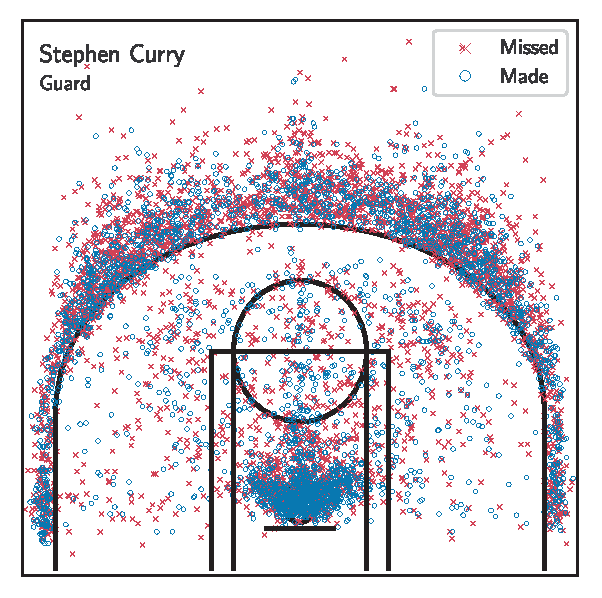
\includegraphics[scale=0.5]{figures/curry_guard.eps}
    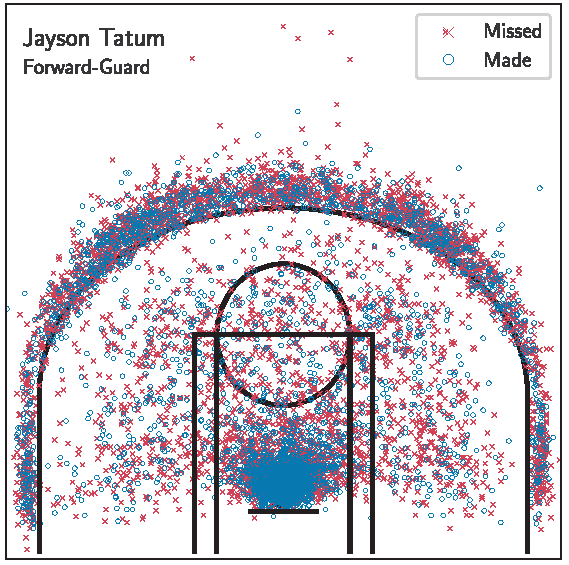
\includegraphics[scale=0.5]{figures/tatum_forward_guard.eps}
    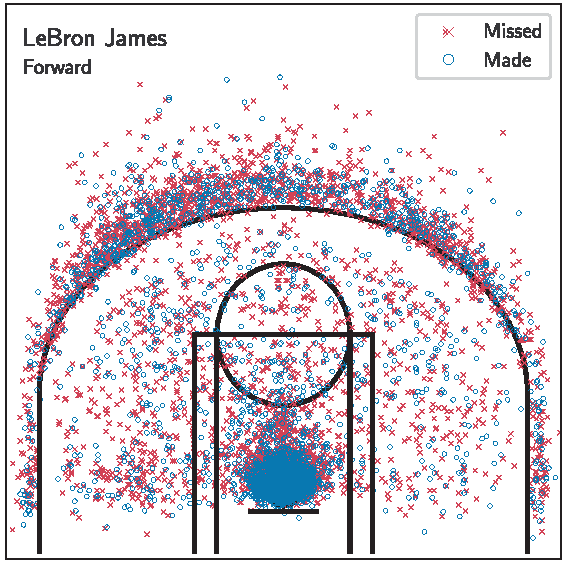
\includegraphics[scale=0.5]{figures/james_forward.eps}
    
\includegraphics[scale=0.5]{figures/embiid_forward_center.eps}
    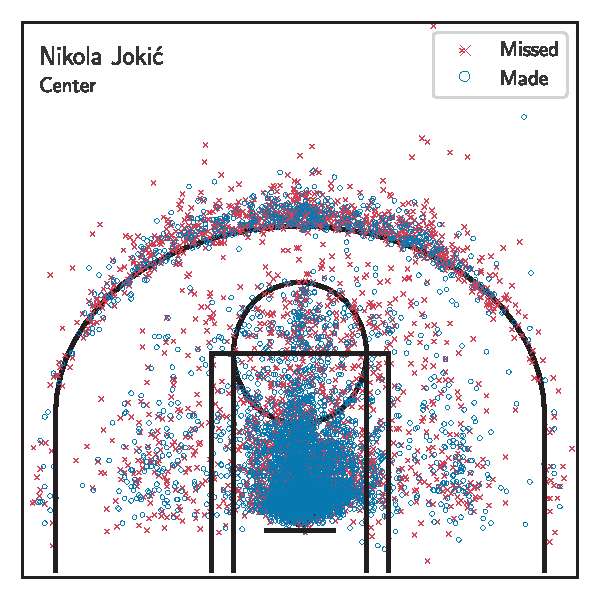
\includegraphics[scale=0.5]{figures/jokic_center.eps}
    \caption{Shots charts for five selected NBA players.}
    \label{fig:examples_shooting_charts}
\end{figure}






% section dataset (end)

%!TEX root=../main.tex
\section{Method} % (fold)
\label{sec:method}

The primary thing to consider to convert the shots charts into functional datasets. To do so, we employed a 2-dimensional kernel density estimation for both the attempted and made shots, utilizing Silverman's rule \cite{silvermanDensityEstimationStatistics1986} for the estimation of the bandwith. The density estimation is conducted on a regularly spaced grid consisting of $201 \times 201$ points. We obtain observations of bivariate functional data, where both features are defined on a two-dimensional rectangular domain, and observed on an equidistant grid of size $201 \times 201$. Figure~\ref{fig:examples_shooting_density} presents the density estimation of the same five players than for the shots charts in Figure~\ref{fig:examples_shooting_charts}. 

\textcolor{red}{The method can be summarized with these steps:
\begin{enumerate}
    \item 2D Kernel density estimation
    \item MFPCA
    \item Clustering
\end{enumerate}}


\textcolor{red}{We estimate the functional principal components using the \texttt{Gram}, \texttt{(Tensor) PCA} and \texttt{2D/1D B-Splines} methods. For the \texttt{Gram} method, we directly use the estimated densities to estimate the eigencomponents. For the \texttt{(Tensor) PCA} method, the estimation of the multivariate eigenimages is based on the univariate estimation of $30$ univariate eigenimages. The estimation of the (univariate) eigenimages is performed with the FCP-TPA where the smoothing parameters are chosen via cross-validation in $[10^{-5}, 10^5]$. For the \texttt{2D/1D B-splines} method, the two components are expanded in tensor products of $13 \times 13$ B-splines. We do not add a smoothing penalty in that case, as the smoothing step is performed in the kernel density estimation.}

\textcolor{red}{Clustering of the scores in the FPCA basis. I would probably use $k$-means with $k = 5$, it makes sense to have $k = 5$ because there are $5$ players of the court.}


\begin{figure}
    \centering
    
\includegraphics[scale=0.35]{figures/curry_density.eps}
    
\includegraphics[scale=0.35]{figures/tatum_density.eps}
    
\includegraphics[scale=0.35]{figures/james_density.eps}
    
\includegraphics[scale=0.35]{figures/embiid_density.eps}
    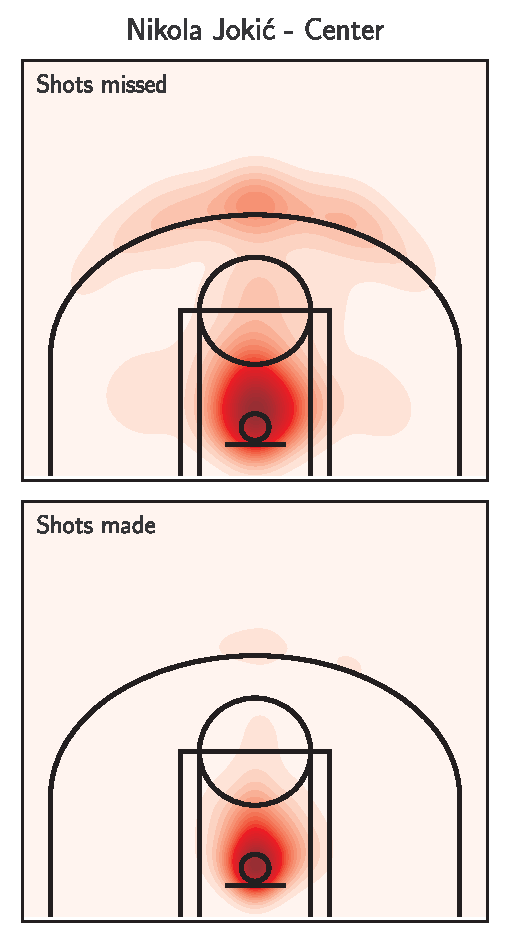
\includegraphics[scale=0.35]{figures/jokic_density.eps}
    \\
    
\includegraphics[scale=0.35]{figures/colorbar.eps}
    \caption{Shots charts density for five selected NBA players. Note that the densities have been individually normalized between $0$ and $1$.}
    \label{fig:examples_shooting_density}
\end{figure}


% section method (end)

%!TEX root=../main.tex
\section{Results} % (fold)
\label{sec:results}

\subsection{Decomposition of the densities} % (fold)
\label{sub:decomposition_of_the_densities}

We apply MFPCA to estimate the mean functions and eigenfunctions, providing a description of player shooting behavior. Figure~\ref{fig:mean_eigenfunctions} presents the estimation of the mean functions alongside the estimated functional principal components, which capture deviations from the mean shooting density. Unlike the shooting densities, the functional principal components may take on negative values as they represent deviations from the mean rather than densities themselves. For presentation purposes, the functional principal components have been normalized between $-1$ and $1$. Blue areas correspond to negative values of the functional components, and thus contribute negatively to the density, while red area corresponds to positive values of the functional components, and thus contribute positively to the density. The mean chart represents the shooting behavior of the average player in the NBA. Shots are most frequently taken in the paint, then the most common position is behind the three-point line, in the wings and the corners. We remark that the elbows and the short-corners are less important as shooting spots. The estimated functional components can be explained as characterising different shooting behaviors. We first note that, except for $\phi_3$, the functional components for missed and made shots are similar. This suggests  that players do not have specific shooting position where the percentage of missed shots significantly exceeds that of made shots. The first component, explained $67.9\%$ of the total variance, contrasts players based on their overall shooting frequency relative to the average NBA player. A player with a positive score $c_1$ for $\phi_1$ will shots more frequently, both successfully and unsuccessfully, than average. These effects are mainly focused on the high-density areas of the court such as the paint and beyond the arc (i.e., $\phi_1$ has a similar shape to the mean function). Conversely, a negative score corresponds to players who shoot less frequently than the average, with effects concentrated in these same regions. The second component (explaining $8.5\%$ of the total variance) highlights a contrast between shooting inside and outside the three-pointer line. Players with a positive score $c_2$ for $\phi_2$ prefer to shoot closer to the basket, while those with negative scores prefer long-range shots. The third component (explaining $6.1\%$ of the total variance) contrasts players that shoot in the paint and the others. Positive scores $c_3$ are associated with frequent attempts and successes in the paint, while negative scores would prefer to shoot farther out. Interestingly, players who perform well near the basket also tend to attempt and miss shots from the corners. The fourth component (explaining $4.0\%$ of the total variance) captures differences between shooting from the wings and shooting along the axis of the hoop. Players with positive (resp. negative) score will shot in the axis of the hoop (resp. from the wing). 
\begin{figure}
    \centering
    
\includegraphics[scale=0.35]{figures/mean.eps}
    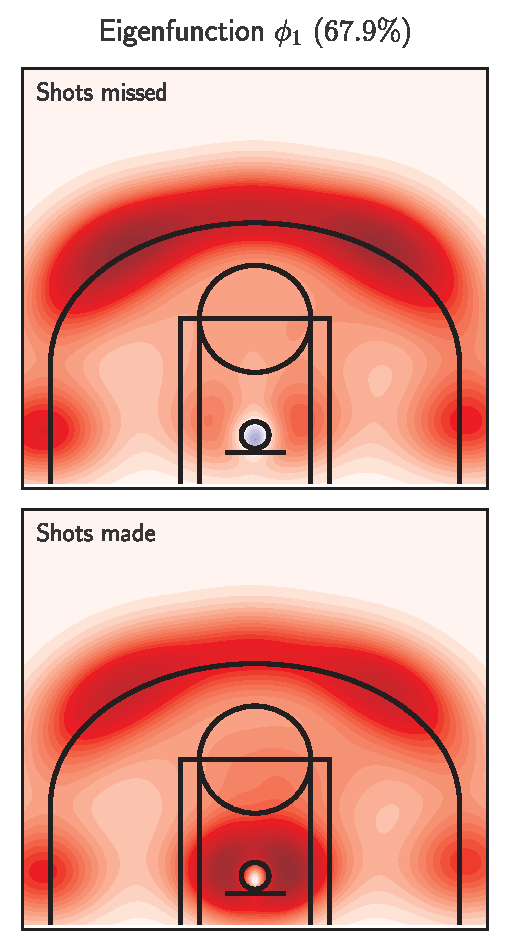
\includegraphics[scale=0.35]{figures/eigenfunction_1.eps}
    
\includegraphics[scale=0.35]{figures/eigenfunction_2.eps}
    
\includegraphics[scale=0.35]{figures/eigenfunction_3.eps}
    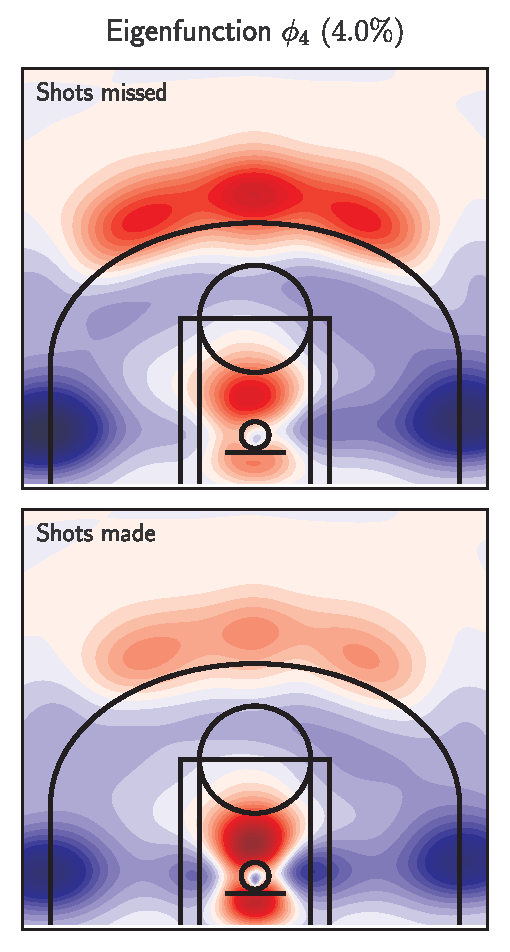
\includegraphics[scale=0.35]{figures/eigenfunction_4.eps}
    \\
    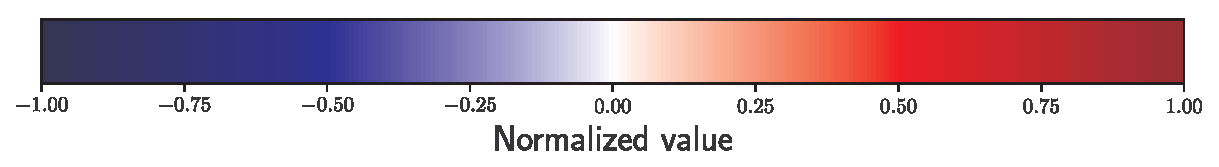
\includegraphics[scale=0.35]{figures/colorbar2.eps}
    \caption{Estimation of the mean surface and the eigenfunctions of the density shots charts. The eigenfunctions represent deviation from the mean surface and are defined up to a sign. Their values at specific points are thus not interpretable \emph{per se}. Note that the mean surface and eigenfunctions have been normalized between $-1$ and $1$ for presentation purpose.}
    \label{fig:mean_eigenfunctions}
\end{figure}

As an example, Figure~\ref{fig:examples_players} presents the decomposition of Stephen Curry. We remark that he shots more than the average player, because he miss and make more shots that the average player, as his first coefficient $c_1$ is positive. He does have a little preference for shooting behind the three-points line as his second coefficient is close to $0$. Its coefficient $c_3$ is a small negative values, indicating that he is around average for this eigenfunction. However, he prefers to shoots in the axis of the basket (positive coefficient $c_4$) compare to the other players. 
\begin{figure}
    \centering
    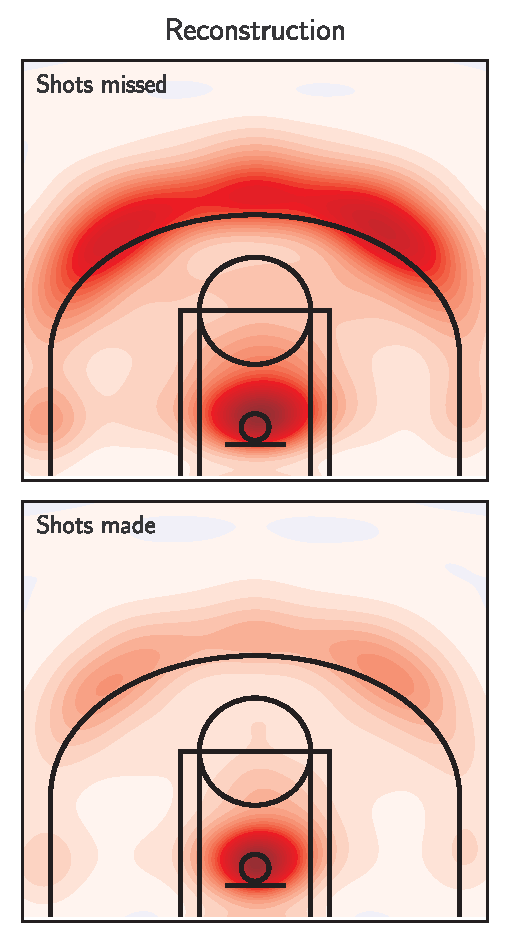
\includegraphics[scale=0.295]{figures/curry_reconstruction.eps}
    
\includegraphics[scale=0.295]{figures/mean.eps}
    
\includegraphics[scale=0.295]{figures/curry_eigenfunction_1.eps}
    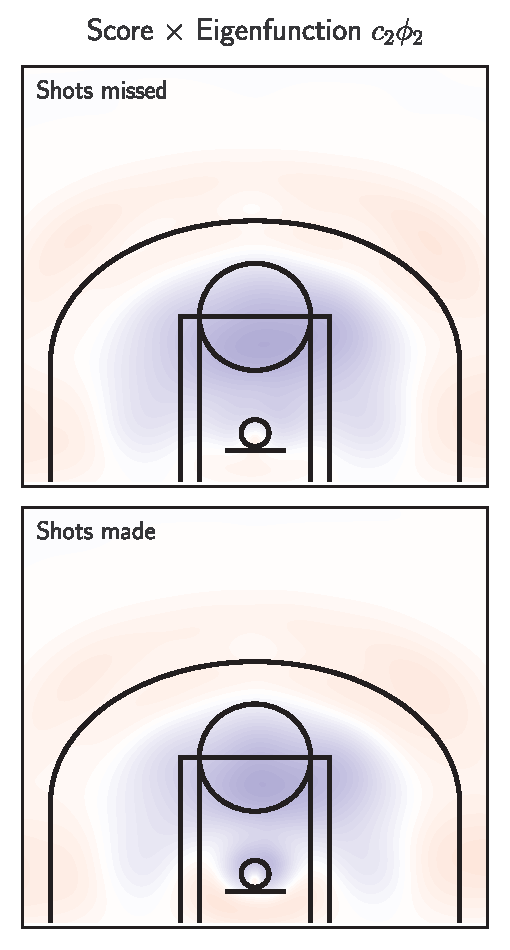
\includegraphics[scale=0.295]{figures/curry_eigenfunction_2.eps}
    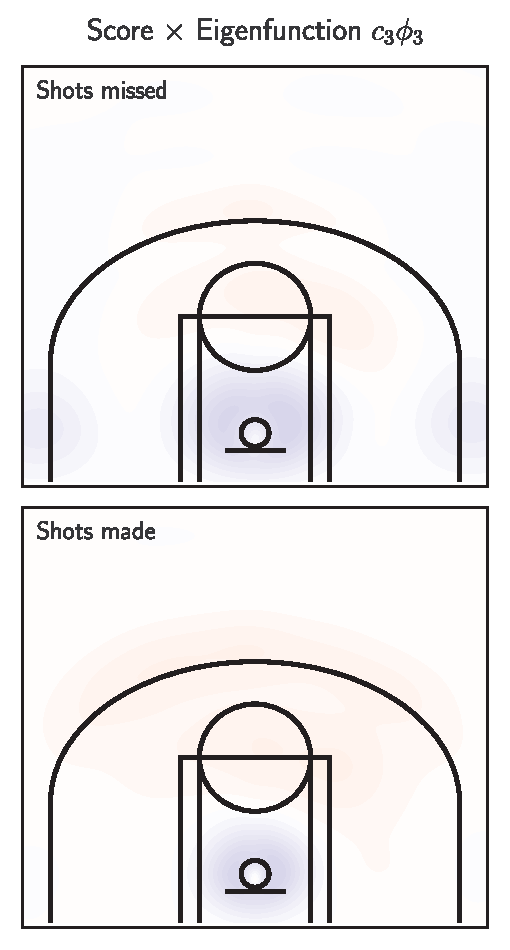
\includegraphics[scale=0.295]{figures/curry_eigenfunction_3.eps}
    
\includegraphics[scale=0.295]{figures/curry_eigenfunction_4.eps}
    \\
    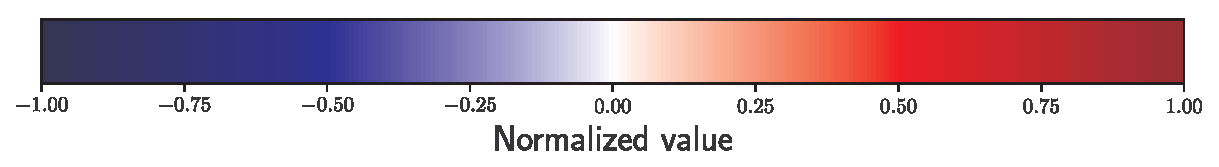
\includegraphics[scale=0.35]{figures/colorbar2.eps}
    \caption{Example of the decomposition of Stephen Curry into the eigenfunctions basis.}
    \label{fig:examples_players}
\end{figure}

Figure~\ref{fig:clusters} presents the estimated scores $c_k$ from~\eqref{eq:kl_decomp} colored by their playing position according to the NBA. We highlight the scores of one player per position. We remark that no score can distinguish the players typology as defined by the NBA as the scores of each position are overlapping one another. From Figure~\ref{fig:clusters}, we remark that some players exhibit scores (coefficients) that are very different than the other players. For example, for the second eigenfunction, Chris Paul (with a large coefficient) and Duncan Robinson (with a large negative coefficient) may be designed as outliers. Similarly, for the third eigenfunction, Chris Paul has a large negative coefficient. It may seems contradictory for Chris Paul, as a positive $c_2$ is explained as a preference for shooting from the painted area and a negative $c_3$ is explained as a preference for shooting from the three-points line. However, this is explained by the fact that the most common shooting position of Chris Paul is the high post (between the three-point line and the painted area), and so the eigenfunctions are compensating each others. This situation is not common in today's NBA. Finally, for the fourth eigenfunction, Reggie Bullock Jr. has a large negative coefficient, indicating a large preference for shooting from the wings and corners.
\begin{figure}
    \centering
    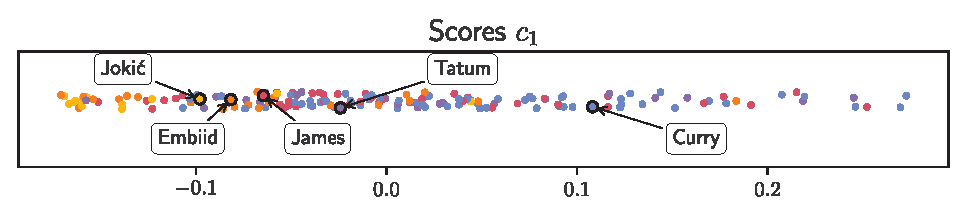
\includegraphics[scale=0.95]{figures/scores_1.eps}
    
\includegraphics[scale=0.95]{figures/scores_2.eps}
    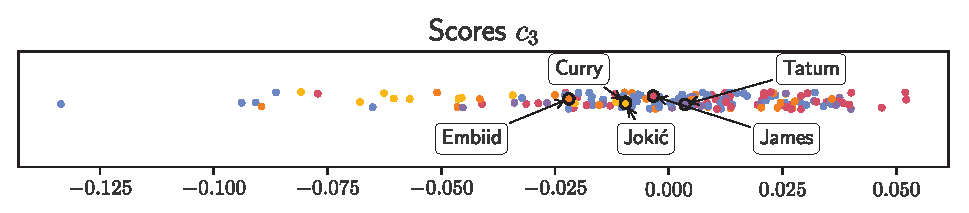
\includegraphics[scale=0.95]{figures/scores_3.eps}
    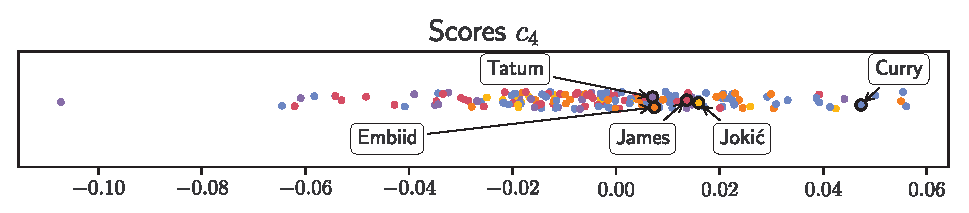
\includegraphics[scale=0.95]{figures/scores_4.eps}
    
\includegraphics[scale=0.95]{figures/legend.eps}
    \caption{Scatter plots of the coefficients colored using the NBA defined typology of players. We highlighted one player per position. The scores have been jittered on the y-axis for visualisation purposes.}
    \label{fig:clusters}
\end{figure}


% subsection decomposition_of_the_densities (end)

\subsection{Clustering} % (fold)
\label{sub:clustering}

The $k$-medoids algorithm has been applied to the coefficients plotted in Figure~\ref{fig:clusters} as described in Section~\ref{sec:method}. We are aiming for $5$ clusters as the number of players on the court for each team. The complete clustering results are given the Appendix~\ref{sec:clustering_results}. To explain the clusters, we compute the mean coefficients per cluster and multiply by the eigenfunctions. It results in the decomposition of the average player within each cluster. The decompositions differ noticeably between the clusters. Figures~\ref{fig:average_cluster_no_weight} and~\ref{fig:average_cluster_weight} represent the decomposition for the average player of each cluster. For the interpretation of each cluster, we recall that the decomposition must be interpreted with respect to an average player, and the eigenfunctions represent a deviation from the mean. 


\begin{figure}
    \centering
    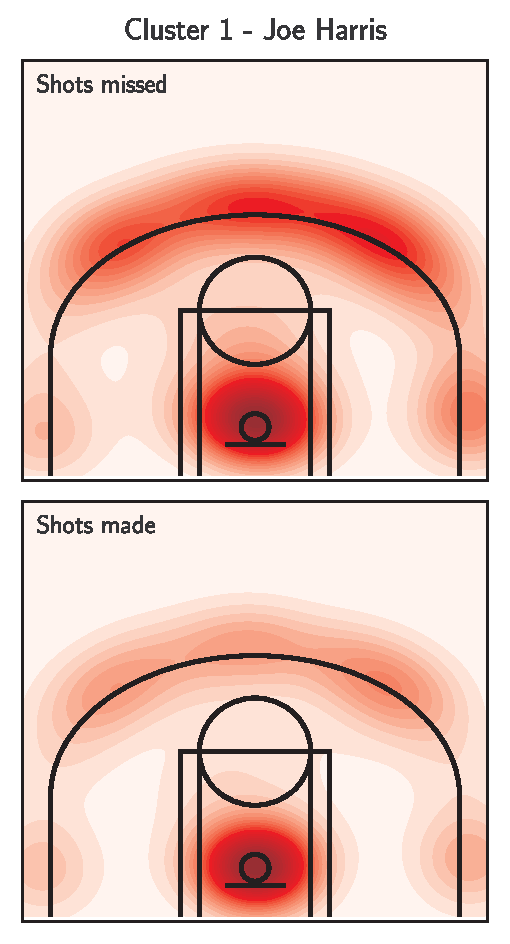
\includegraphics[scale=0.35]{figures/average_player_1.eps}
    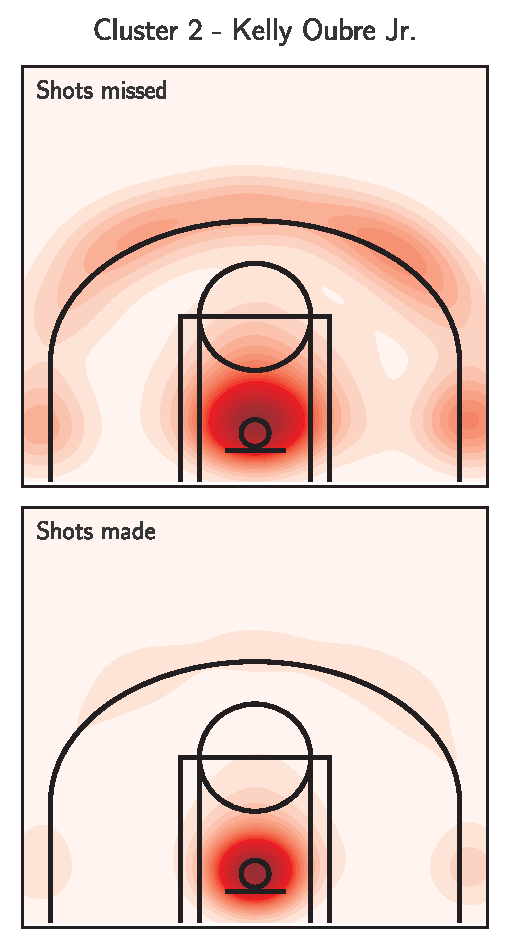
\includegraphics[scale=0.35]{figures/average_player_2.eps}
    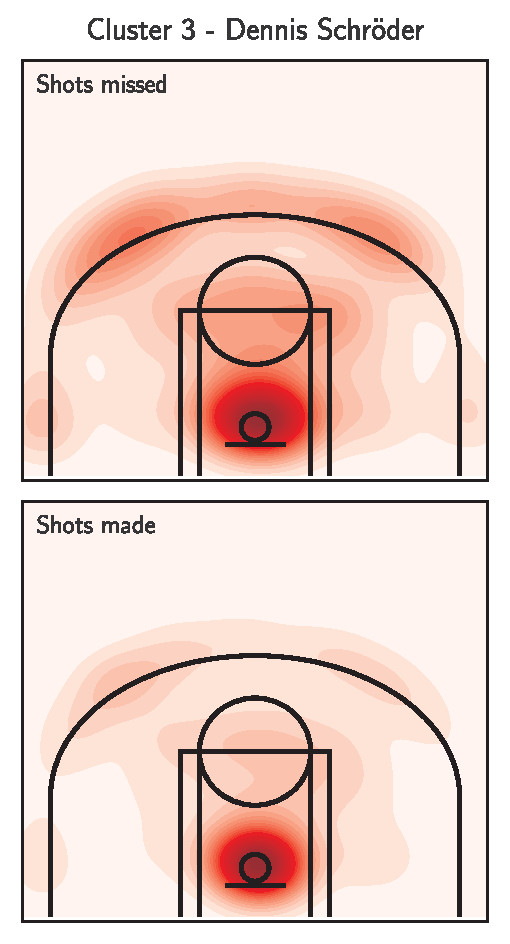
\includegraphics[scale=0.35]{figures/average_player_3.eps}
    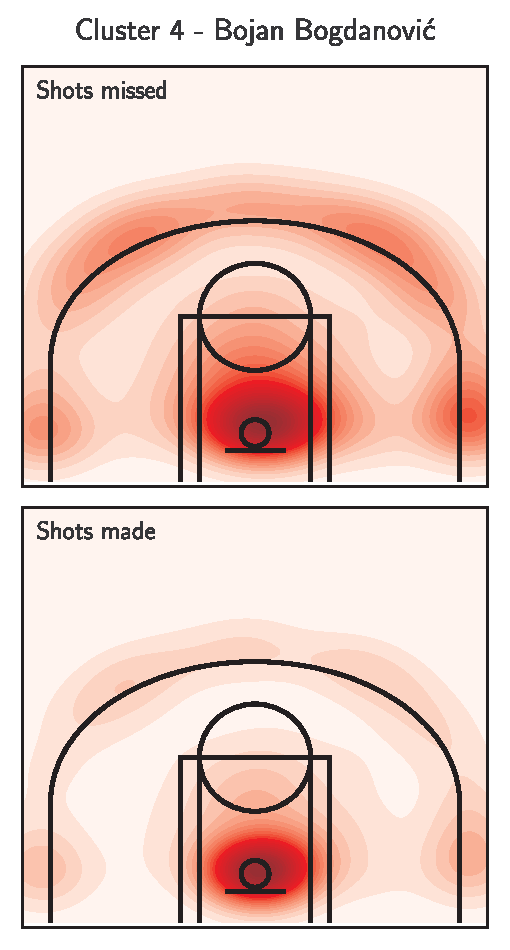
\includegraphics[scale=0.35]{figures/average_player_4.eps}
    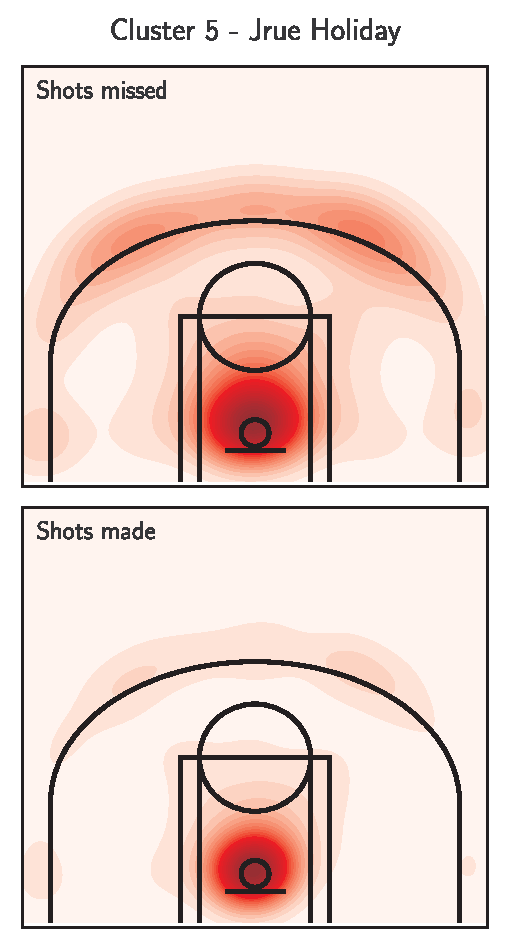
\includegraphics[scale=0.35]{figures/average_player_5.eps}
    \caption{Most representative player of each cluster.}
    \label{fig:average_cluster_no_weight}
\end{figure}

\begin{figure}
    \centering
    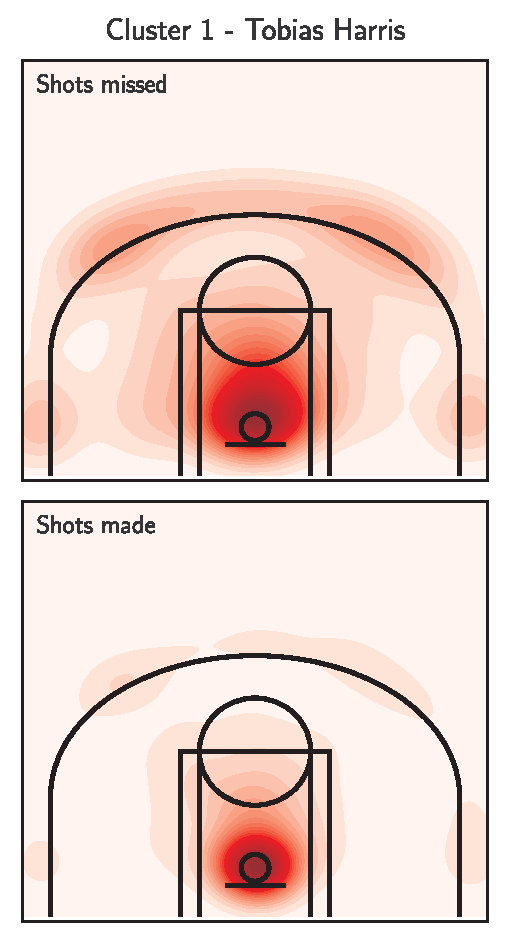
\includegraphics[scale=0.35]{figures/average_player_1_weighted.eps}
    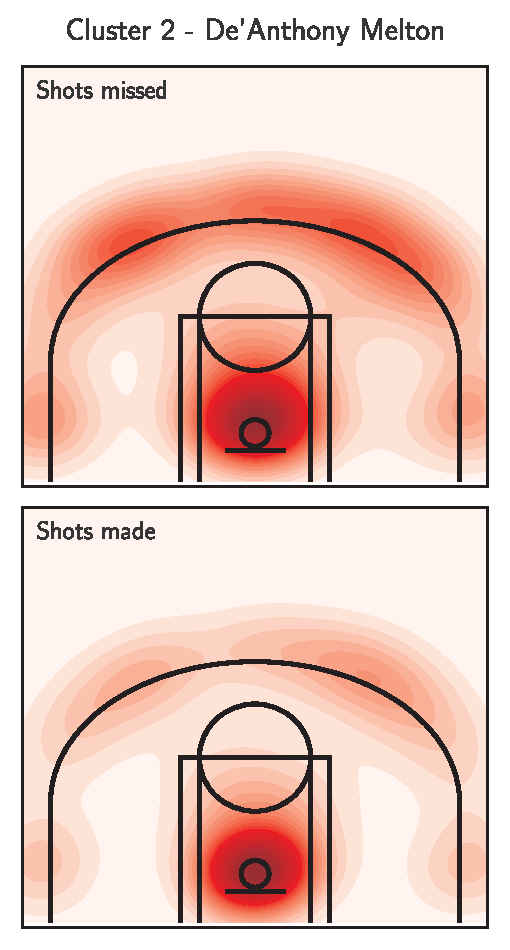
\includegraphics[scale=0.35]{figures/average_player_2_weighted.eps}
    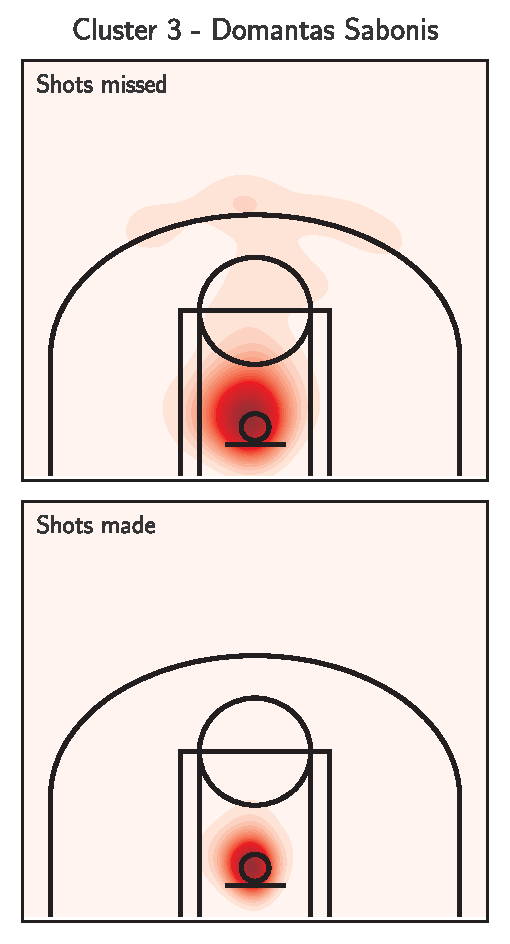
\includegraphics[scale=0.35]{figures/average_player_3_weighted.eps}
    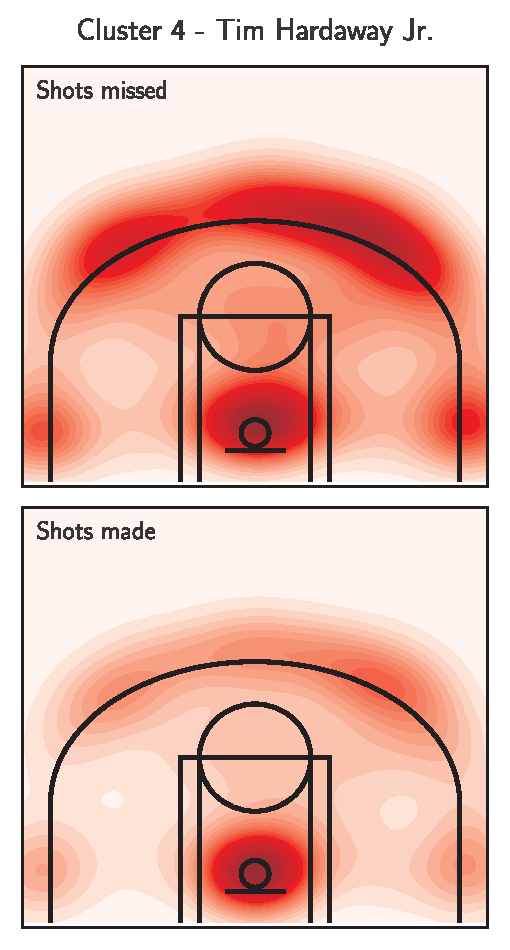
\includegraphics[scale=0.35]{figures/average_player_4_weighted.eps}
    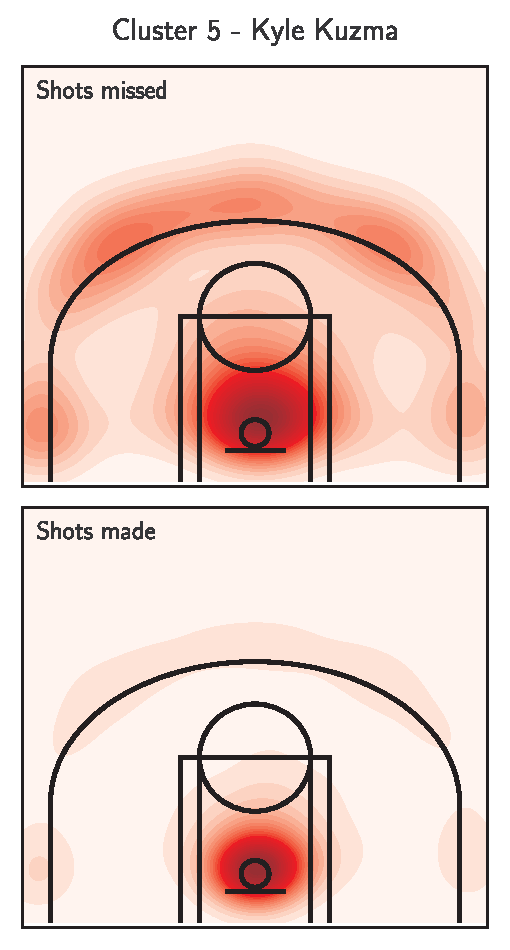
\includegraphics[scale=0.35]{figures/average_player_5_weighted.eps}
    \caption{Most representative player of each cluster.}
    \label{fig:average_cluster_weight}
\end{figure}


\begin{figure}
    \centering
    \begin{subfigure}{0.32\textwidth}
        \centering
        
\includegraphics[scale=0.5]{figures/confusion_mat_kmedoids_no_weights.eps}
        \caption{NBA / No weights.}
    \end{subfigure}
    \hfill
    \begin{subfigure}{0.32\textwidth}
        \centering
        
\includegraphics[scale=0.5]{figures/confusion_mat_kmedoids_weights.eps}
        \caption{NBA / Weights.}
    \end{subfigure}
    \hfill
    \begin{subfigure}{0.32\textwidth}
        \centering
        
\includegraphics[scale=0.5]{figures/confusion_matk_medoids_w_no_w.eps}
        \caption{Weights / No weights}
    \end{subfigure}
    \caption{Confusion matrices.}
    \label{fig:confusion_mat}
\end{figure}




% \begin{table}
% \centering
% \caption{Example of players in each clusters}
% \label{tab:example_players_clusters}
% \begin{tabular}{ cccccc } 
%  Cluster 1 & Cluster 2 & Cluster 3 & Cluster 4 & Cluster 5 \\ 
%  \hline
%  B. Adebayo & S. Curry & D. Boker & J. Crowder &  L. James \\
%  G. Antetokounmpo & E. Fournier & L. Dončić & J. Holiday & N. Jokić \\
%  B. Simmons & K. Love & J. Harden & P. Mills & J. Tatum \\
%  R. Gobert & K. Lowry & K. Irving & D. Robinson & K.-A. Towns \\
%  M. Robinson & C. Paul & K. Leonard & L. Shamet & J. Embiid \\
% \end{tabular}
% \end{table}

% From Figure~\ref{fig:clusters_1}, the average player in cluster $1$ tend to shot less than the other players (coefficient from the first eigenfunction is negative).
% \begin{figure}
%     \centering
%     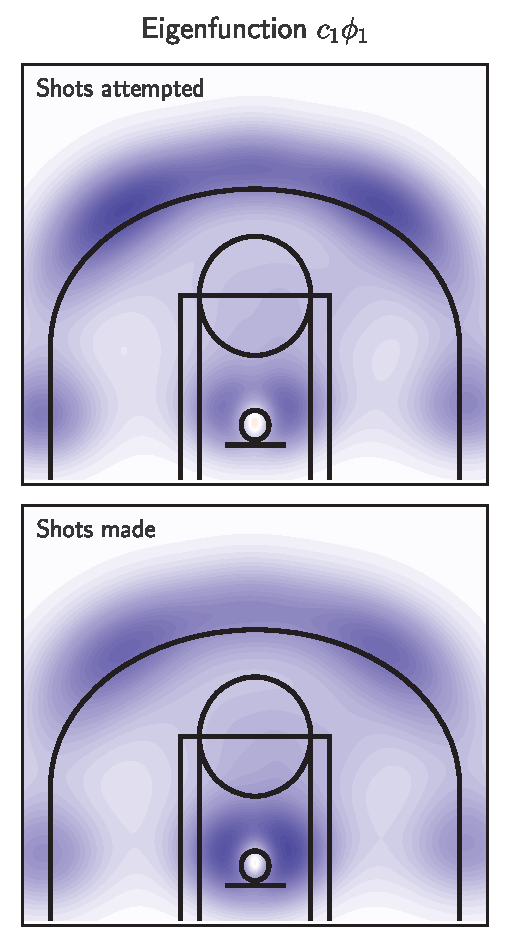
\includegraphics[scale=0.4]{figures/cluster_1_eigenfunction_1.eps}
%     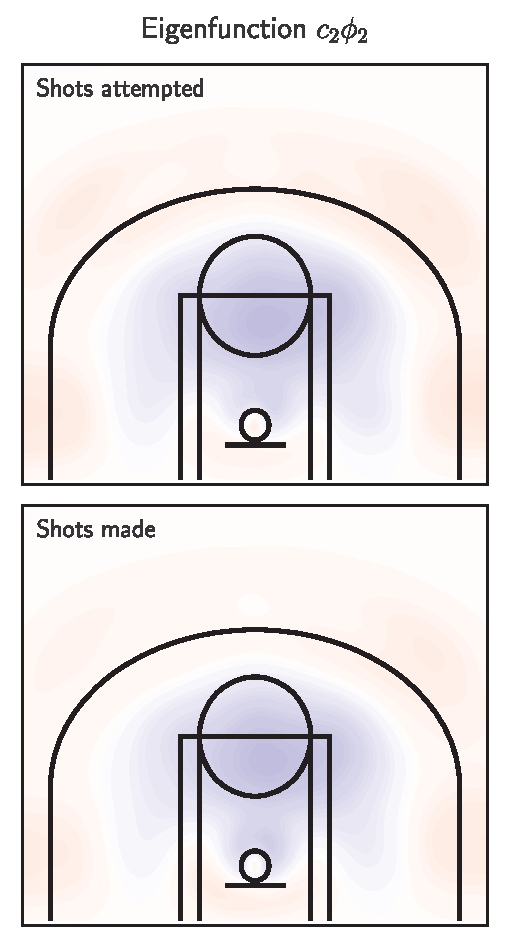
\includegraphics[scale=0.4]{figures/cluster_1_eigenfunction_2.eps}
%     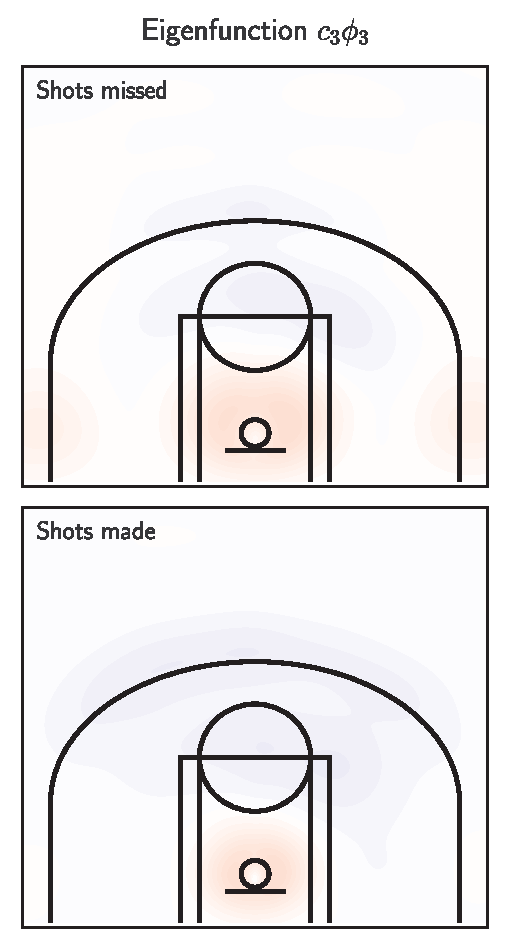
\includegraphics[scale=0.4]{figures/cluster_1_eigenfunction_3.eps}
%     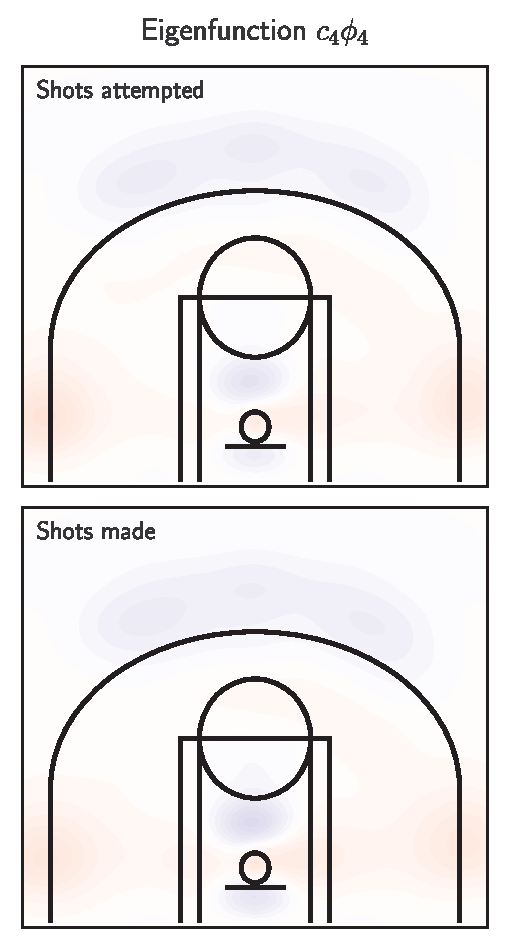
\includegraphics[scale=0.4]{figures/cluster_1_eigenfunction_4.eps}
%     \caption{Cluster 1}
%     \label{fig:clusters_1}
% \end{figure}

% From Figure~\ref{fig:clusters_2}, the average player in cluster $2$ tend to shot more than the other players (coefficient from the first eigenfunction is positive). These players do not have shooting preference as the coefficients of the second to fourth eigenfunctions is close to $0$.
% \begin{figure}
%     \centering
%     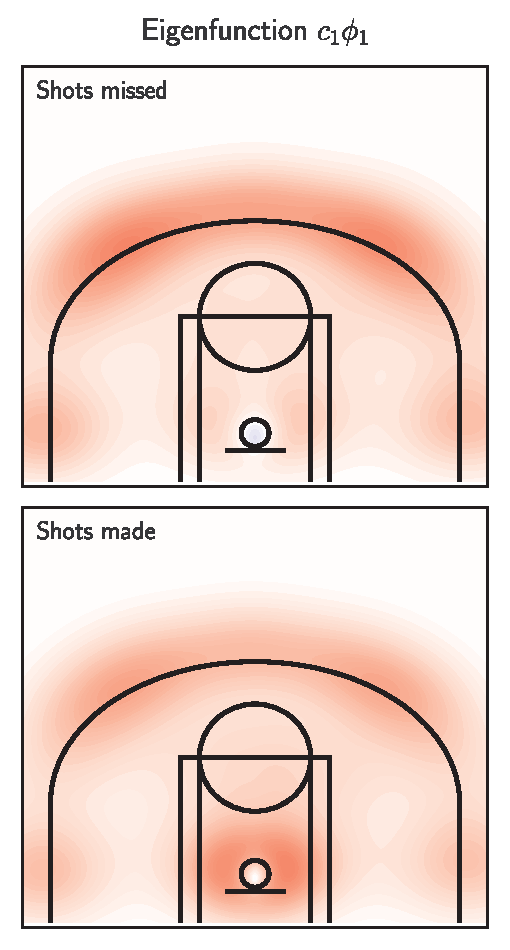
\includegraphics[scale=0.4]{figures/cluster_2_eigenfunction_1.eps}
%     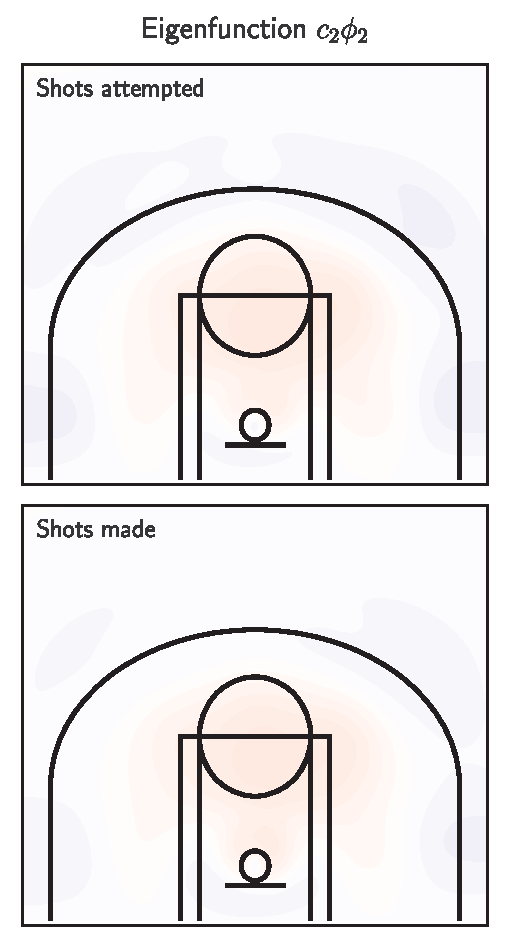
\includegraphics[scale=0.4]{figures/cluster_2_eigenfunction_2.eps}
%     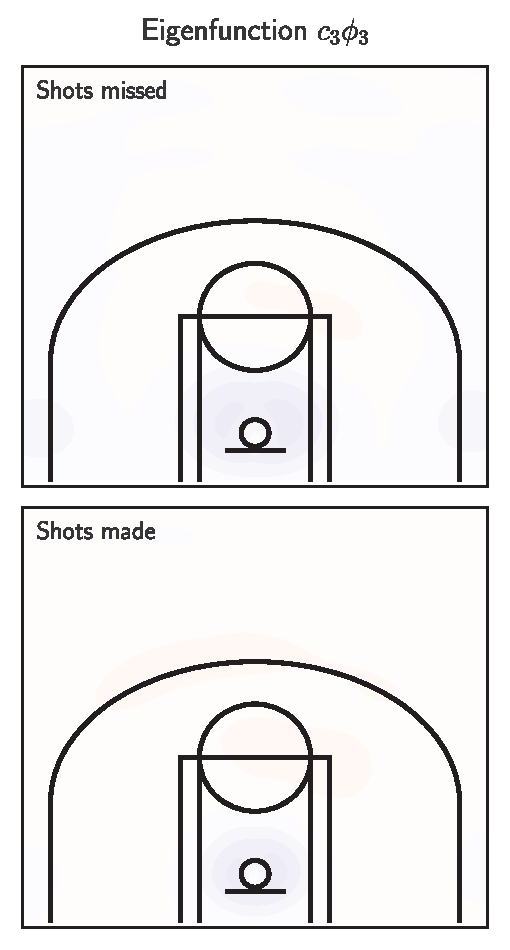
\includegraphics[scale=0.4]{figures/cluster_2_eigenfunction_3.eps}
%     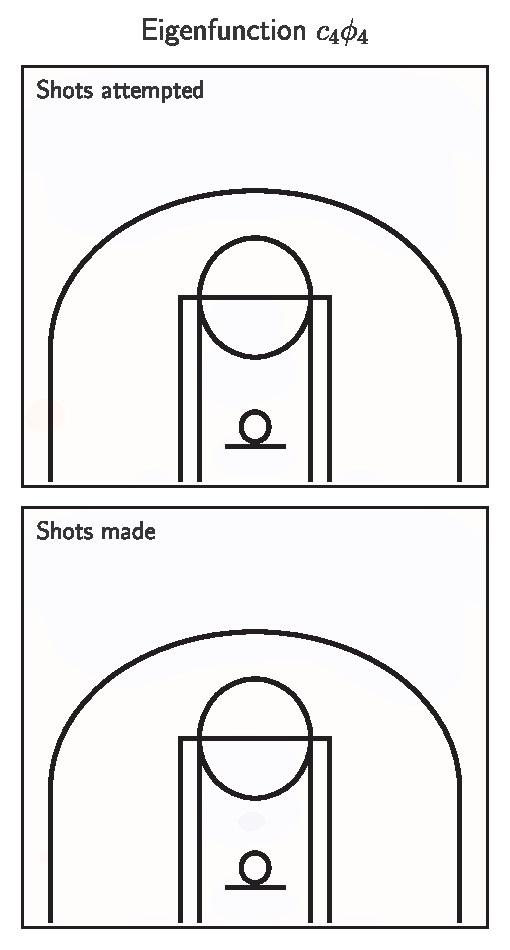
\includegraphics[scale=0.4]{figures/cluster_2_eigenfunction_4.eps}
%     \caption{Cluster 2}
%     \label{fig:clusters_2}
% \end{figure}

% From Figure~\ref{fig:clusters_3}, players in cluster $3$ are average players in the NBA. Their coefficients for each eigenfunction is close to $0$.
% \begin{figure}
%     \centering
%     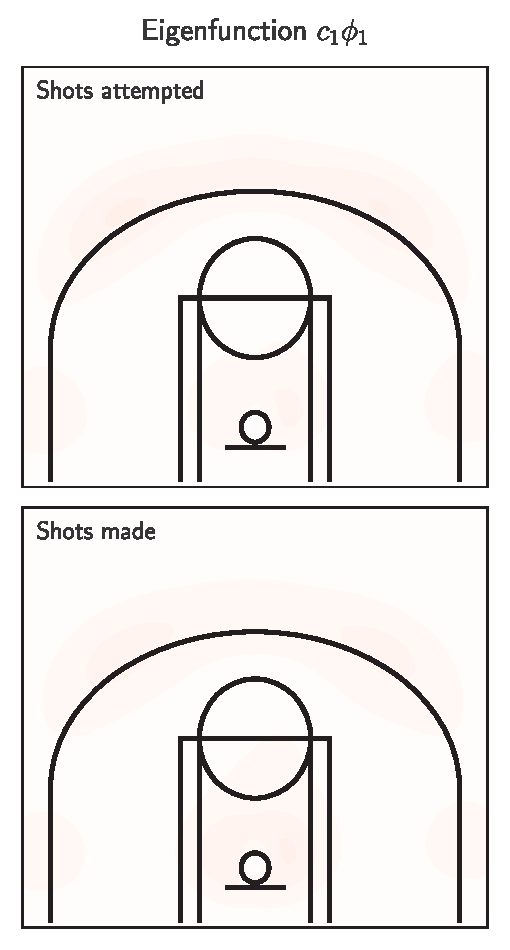
\includegraphics[scale=0.4]{figures/cluster_3_eigenfunction_1.eps}
%     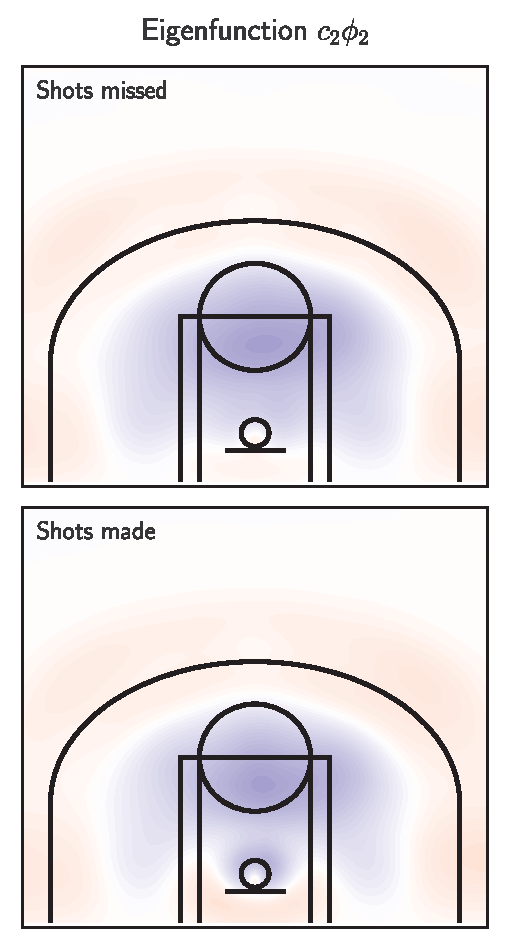
\includegraphics[scale=0.4]{figures/cluster_3_eigenfunction_2.eps}
%     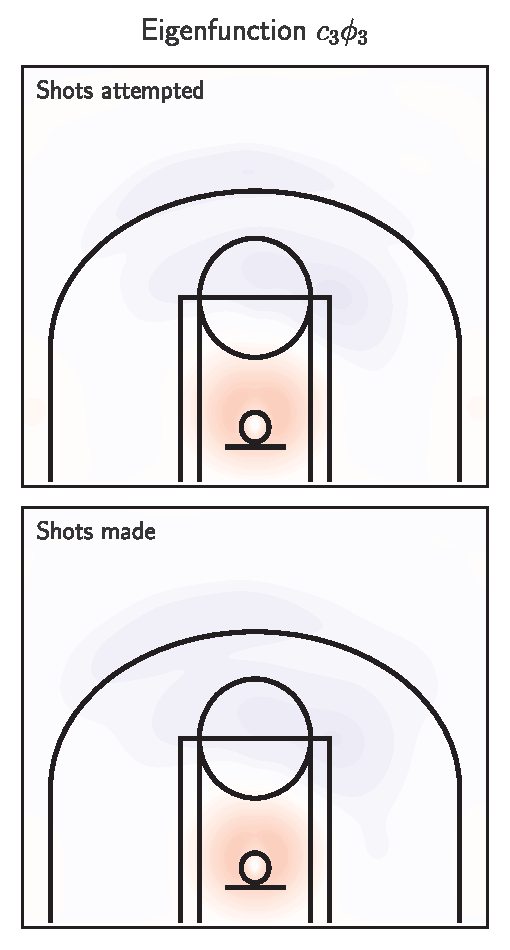
\includegraphics[scale=0.4]{figures/cluster_3_eigenfunction_3.eps}
%     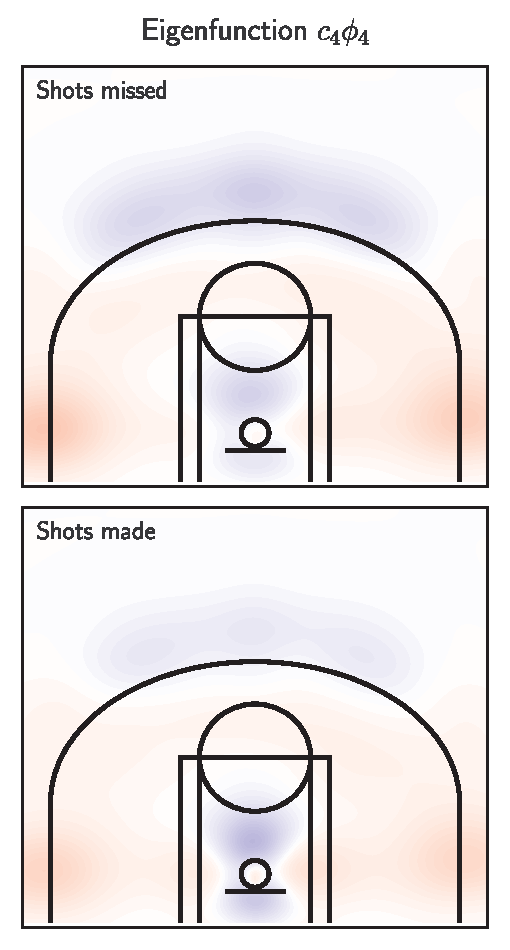
\includegraphics[scale=0.4]{figures/cluster_3_eigenfunction_4.eps}
%     \caption{Cluster 3}
%     \label{fig:clusters_3}
% \end{figure}

% From Figure~\ref{fig:clusters_4}, the average player in cluster $4$ shots more than the other player in the NBA (large positive coefficient). They prefer to shots 3-pointers than 2-pointers (negative coefficients for $\phi_2$ and $\phi_3$). They also prefer to shot in the corners (negative coefficients for $\phi_4$).
% \begin{figure}
%     \centering
%     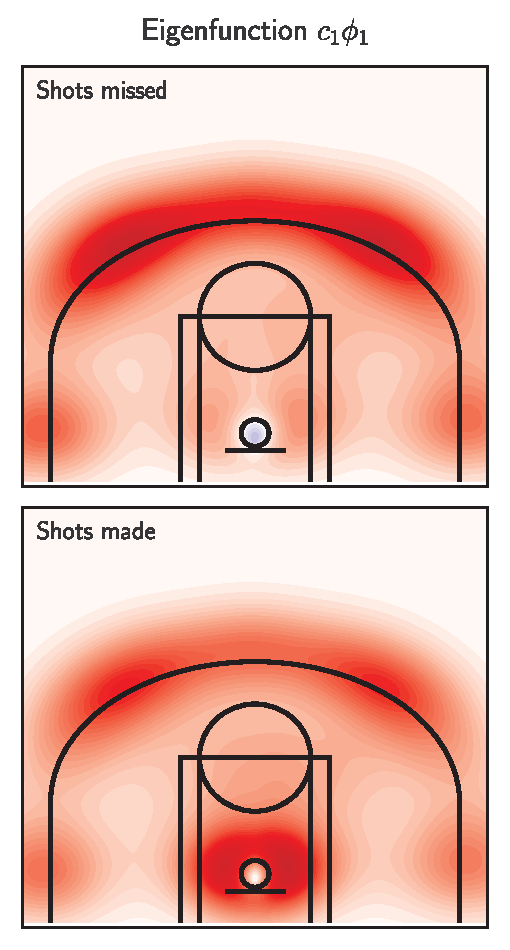
\includegraphics[scale=0.4]{figures/cluster_4_eigenfunction_1.eps}
%     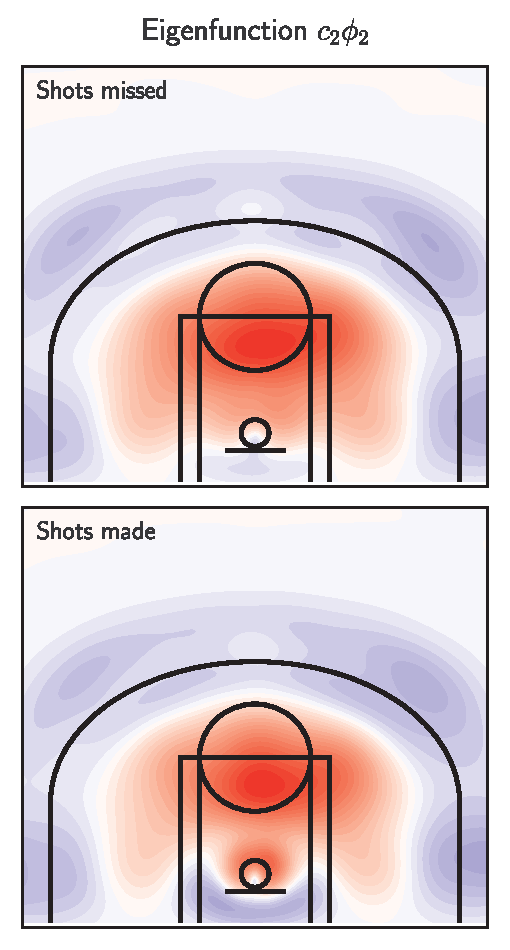
\includegraphics[scale=0.4]{figures/cluster_4_eigenfunction_2.eps}
%     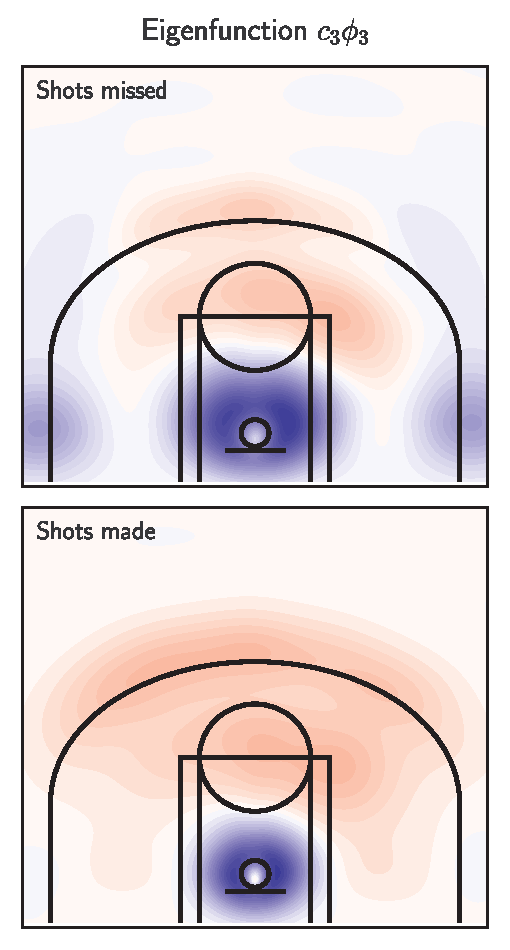
\includegraphics[scale=0.4]{figures/cluster_4_eigenfunction_3.eps}
%     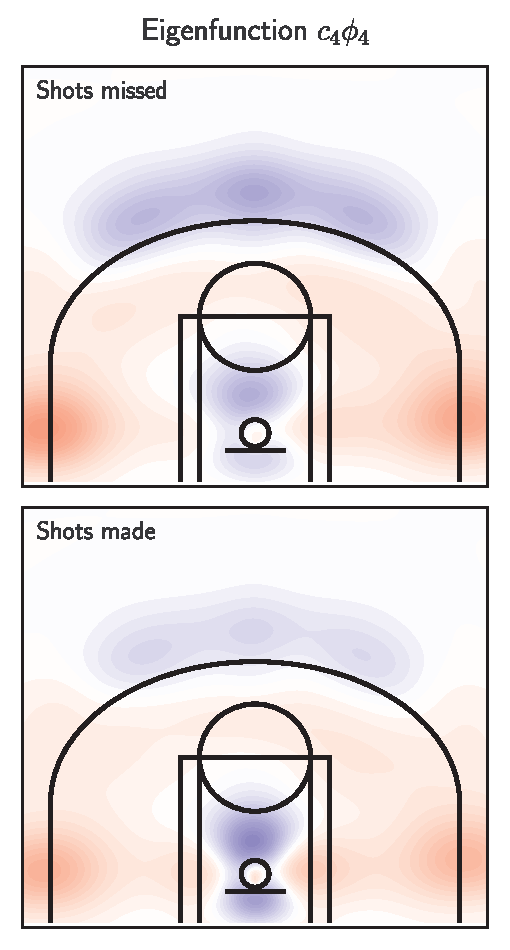
\includegraphics[scale=0.4]{figures/cluster_4_eigenfunction_4.eps}
%     \caption{Cluster 4}
%     \label{fig:clusters_4}
% \end{figure}

% Players from the last cluster (see Figure~\ref{fig:clusters_5}) shot less than  the average NBA player without any particular preference for any position.
% \begin{figure}
%     \centering
%     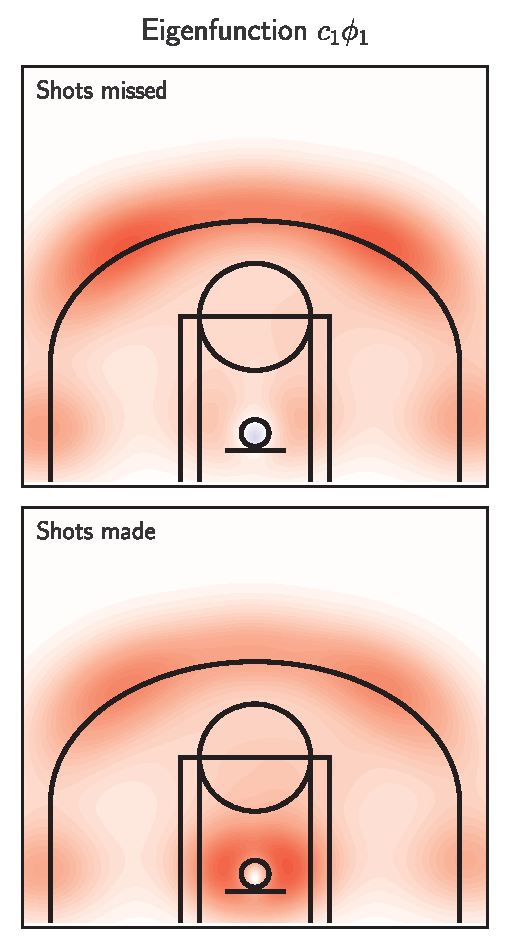
\includegraphics[scale=0.4]{figures/cluster_5_eigenfunction_1.eps}
%     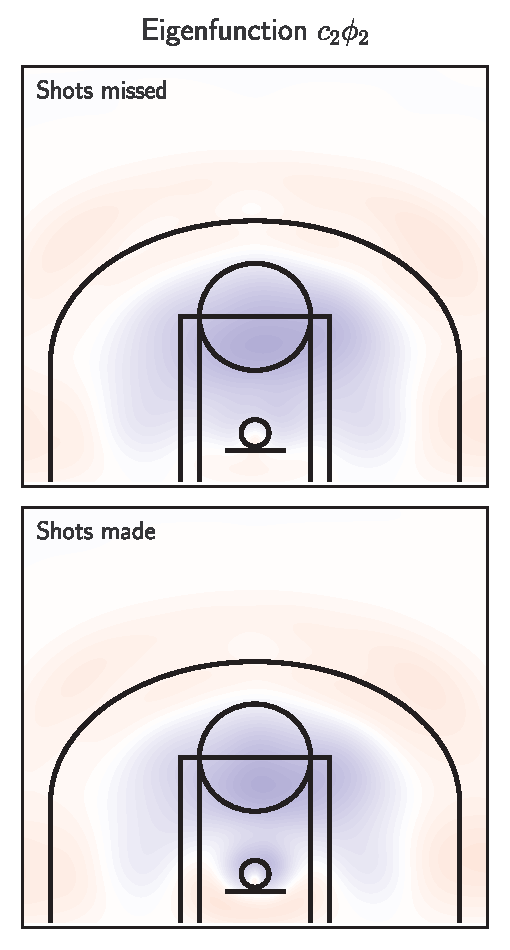
\includegraphics[scale=0.4]{figures/cluster_5_eigenfunction_2.eps}
%     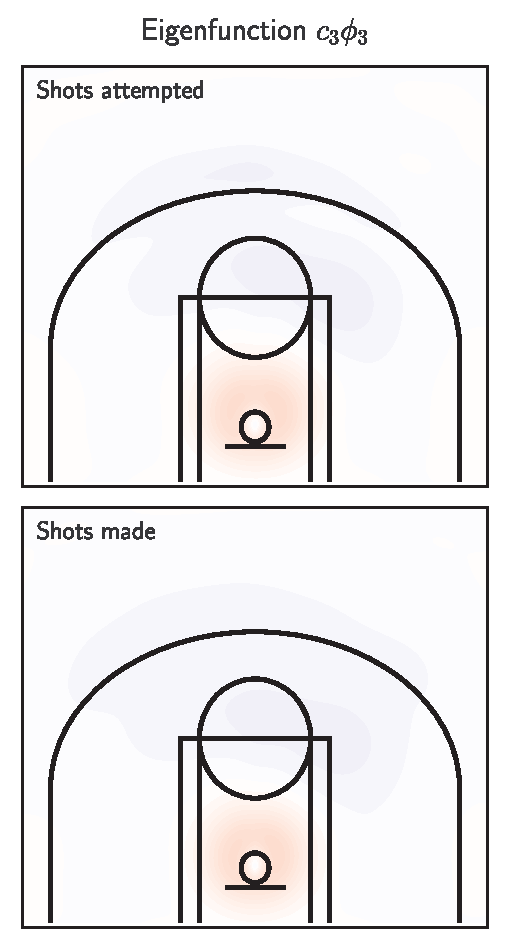
\includegraphics[scale=0.4]{figures/cluster_5_eigenfunction_3.eps}
%     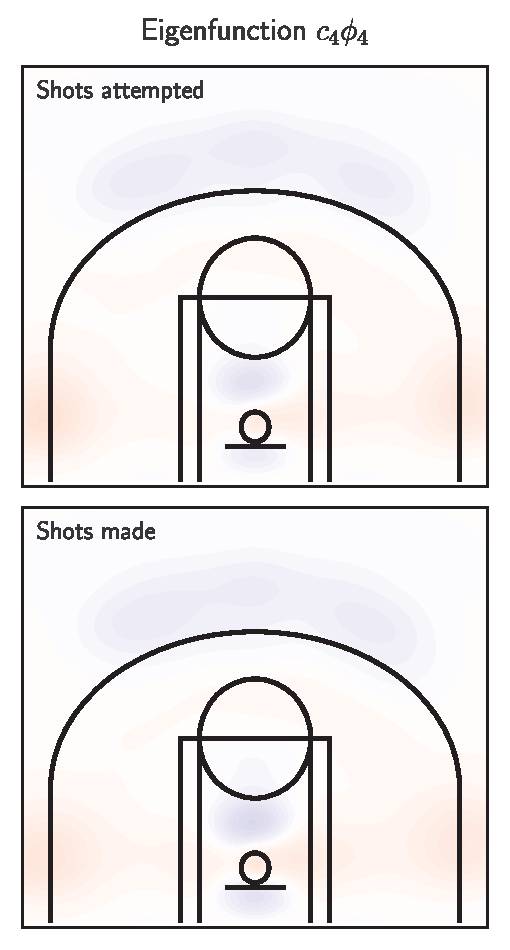
\includegraphics[scale=0.4]{figures/cluster_5_eigenfunction_4.eps}
%     \caption{Cluster 5}
%     \label{fig:clusters_5}
% \end{figure}

% subsection clustering (end)

% section results (end)

%!TEX root=../main.tex
\section{Discussion} % (fold)
\label{sec:discussion}

n this work, we presented a novel representation of NBA players’ shot density charts based on Functional Data Analysis (FDA). We defined the smoothed densities of each player’s made and missed shots as functional data over the entire offensive half-court. This functional representation enabled a principal component decomposition, in which a player’s variation from the mean shot chart is parsimoniously described by a common set of principal component functions, weighted by player-specific scores.

We first used these principal component functions to describe the major modes of variation in shooting behavior. The first component, which explained almost $70\%$ of the total variance, primarily captured shooting frequency, distinguishing between players who shoot with high and low volumes. The remaining components, which explained successively less variation, captured increasingly subtle but interpretable features of shot selection.

We then applied k-medoids clustering to the player-specific scores to construct a data-driven taxonomy of player shooting tendencies. The resulting clusters revealed diverse shooting profiles, which we interpreted through average component scores within each group.

Interestingly, the estimated clusters showed only weak agreement with the conventional NBA-defined player positions. This may be because shooting behavior represents only one aspect of a player’s role; play-making, defensive responsibilities, and off-the-ball movement also influence positional classification. Nevertheless, our analysis provides a novel data-driven perspective on how players differ in their shooting behaviors.

We envision a number of potential uses of both our functional shot-chart representation and the subsequent clustering of shooting patterns.
Firstly, the functional representation of a players shot-chart provides a comprehensive characterization of a player's shooting behavior, i.e., the shot chart is not reduced to one or more scalar summaries.
This representation could be used by coaches or front-office staff to monitor changes in a player's shooting patterns between or within seasons, to identify player-specific tendencies which inform specific training regimes, and also to identify players whose characteristics match the needs of the team during scouting and recruitment.
Because the charts are can naturally be presented in a way that is interpretable to basketball fans who may not be familiar with the underlying mathematics and statistics, the representation can be used to tell stories to the general public about player tendencies, and enable historical comparisons between players, enriching the narrative around the sport.
While we used shots made and shots missed, other metrics defined over the offensive half-court (e.g., shooting efficiency), could be represented in the same way for the aforementioned purposes.

There are a number of possible methodological extensions to the modeling framework.
One of the most exiting avenues is to combine the shot-chart representations with other high-throughput data sources that are now routinely collected within the NBA. 
For example, temporal biomechanical data are now being measured by motion-tracking systems such as Hawk-Eye, and the possibility of a multi-modal representation that reflects a players tactical and physical tendencies -- and the interaction between them -- could provide more detailed and specific analyses.
The models could also be applied in other sports, for example, to characterize a player's typical position in soccer.

{\color{red}Add references}

% {\color{red}In-season use -- is a player's pattern changing?}

% As an extension, use the defensive shot chart from \cite{franksCharacterizingSpatialStructure2015}.

% As an extension, use the shots efficiency and frequency and not shots attempted and made.


% \textcolor{red}{
% The practical applications of analyzing basketball shooting patterns using functional data analysis and clustering can significantly enhance various aspects of player development, coaching strategies, and team performance. Here’s a detailed exploration of these applications:}

% \textcolor{red}{
% **1. Player Development:**
%    - **Tailored Training Programs:** By identifying specific shooting patterns and inefficiencies, coaches can design personalized training regimens that focus on improving weak areas. For example, if a player's analysis shows a lower shooting percentage from certain court locations, targeted drills can be implemented to enhance their skills in those areas.
%    - **Biomechanical Adjustments:** Insights from functional data analysis can help players refine their shooting mechanics. Understanding the optimal release angles, velocities, and body positioning can lead to improved shooting accuracy. For instance, adjusting the release height or speed based on biomechanical feedback can enhance performance[1][3].}

% \textcolor{red}{
% **2. Coaching Strategies:**
%    - **Game Preparation:** Coaches can utilize shooting pattern analyses to prepare specific game strategies against opponents. By studying the shooting tendencies of opposing players, coaches can develop defensive schemes that effectively limit high-percentage shots from preferred locations[2][4].
%    - **In-Game Adjustments:** Real-time data analysis during games allows coaches to make informed decisions about substitutions or play calls based on player performance metrics. For example, if a player is consistently missing shots from a particular area, they may be advised to alter their shot selection or take a break to reassess their approach.}

% \textcolor{red}{
% **3. Team Performance Optimization:**
%    - **Shot Selection Analysis:** Teams can analyze collective shooting data to determine the most effective shot selections during games. This includes evaluating the success rates of different shot types (e.g., three-pointers vs. mid-range shots) and making strategic decisions about when to attempt specific shots based on situational context[4][5].
%    - **Enhanced Scouting Reports:** Detailed analyses of shooting patterns allow for more comprehensive scouting reports on both players and teams. This information can be invaluable for identifying potential trade targets or assessing the strengths and weaknesses of upcoming opponents[2][3].}

% \textcolor{red}{
% **4. Fan Engagement and Analytics:**
%    - **Visualizations for Fans:** Shot charts and other visual analytics tools can be used to engage fans by providing deeper insights into player performances and game strategies. This not only enhances the viewing experience but also fosters a greater understanding of the game among fans[2][4].
%    - **Data-Driven Storytelling:** Teams and analysts can leverage shooting data to tell compelling stories about player development, game trends, and historical comparisons, enriching the narrative around the sport.}


% \textcolor{red}{
% 1. Biomechanics of the Basketball Jump Shot: This source discusses how biomechanics impact shooting performance and provides insights into effective training methods that could be informed by data analysis[1].
% 2. A Model-Based Approach to Shot Charts Estimation in Basketball: This paper outlines advanced methodologies for estimating shot patterns and emphasizes the importance of accurate visualizations in basketball analytics[2].
% 3. New Technology Changing NBA Shooting: This article highlights how emerging technologies are revolutionizing player training through detailed biomechanical analysis, which complements functional data analysis approaches[3].
% 4. Shot Distribution in the NBA: This research examines how shot patterns have evolved over time in relation to rule changes like the three-point line, offering valuable context for current shooting trends[4].
% 5. Using Data to Investigate NBA Shot Patterns: This project demonstrates practical applications of data science in analyzing NBA shooting data, providing insights into shooter accuracy relative to distance and defensive pressure[5].}

% Citations:
% [1] https://www.physio-pedia.com/Biomechanics_of_the_Basketball_Jump_Shot
% [2] https://arxiv.org/html/2405.01182v1
% [3] https://www.espn.co.uk/nba/story/_/id/38042314/i-thought-was-very-informative-new-technology-change-nba-shooting-forever
% [4] https://link.springer.com/article/10.1007/s12662-020-00690-7
% [5] https://nycdatascience.com/blog/student-works/using-data-to-investigate-nba-shot/
% [6] https://www.stat.uga.edu/sites/default/files/Bradley_Lecture%20II.pdf
% [7] https://www.ncbi.nlm.nih.gov/pmc/articles/PMC9494817/
% [8] https://www.frontiersin.org/journals/psychology/articles/10.3389/fpsyg.2022.917980/full

% section discussion (end)


% ACKNOWLEDGMENT -------
\section*{Acknowledgment}

S. Golovkine is partially supported by Science Foundation Ireland under Grant No. 19/FFP/7002 and co-funded under the European Regional Development Fund.

% REFERENCES ---------
\bibliographystyle{apalike}
\bibliography{./biblio.bib}

\end{document}

